\label{sec:incame}

In this section, we firstly give a brief introduction to ROS\cite{quigley2009ros}. To solve the hardware resources conflicts in ROS, we propose the INCMAE framework for ROS softwares to share the CNN accelerator.

\begin{figure*}[t]
	\centering
    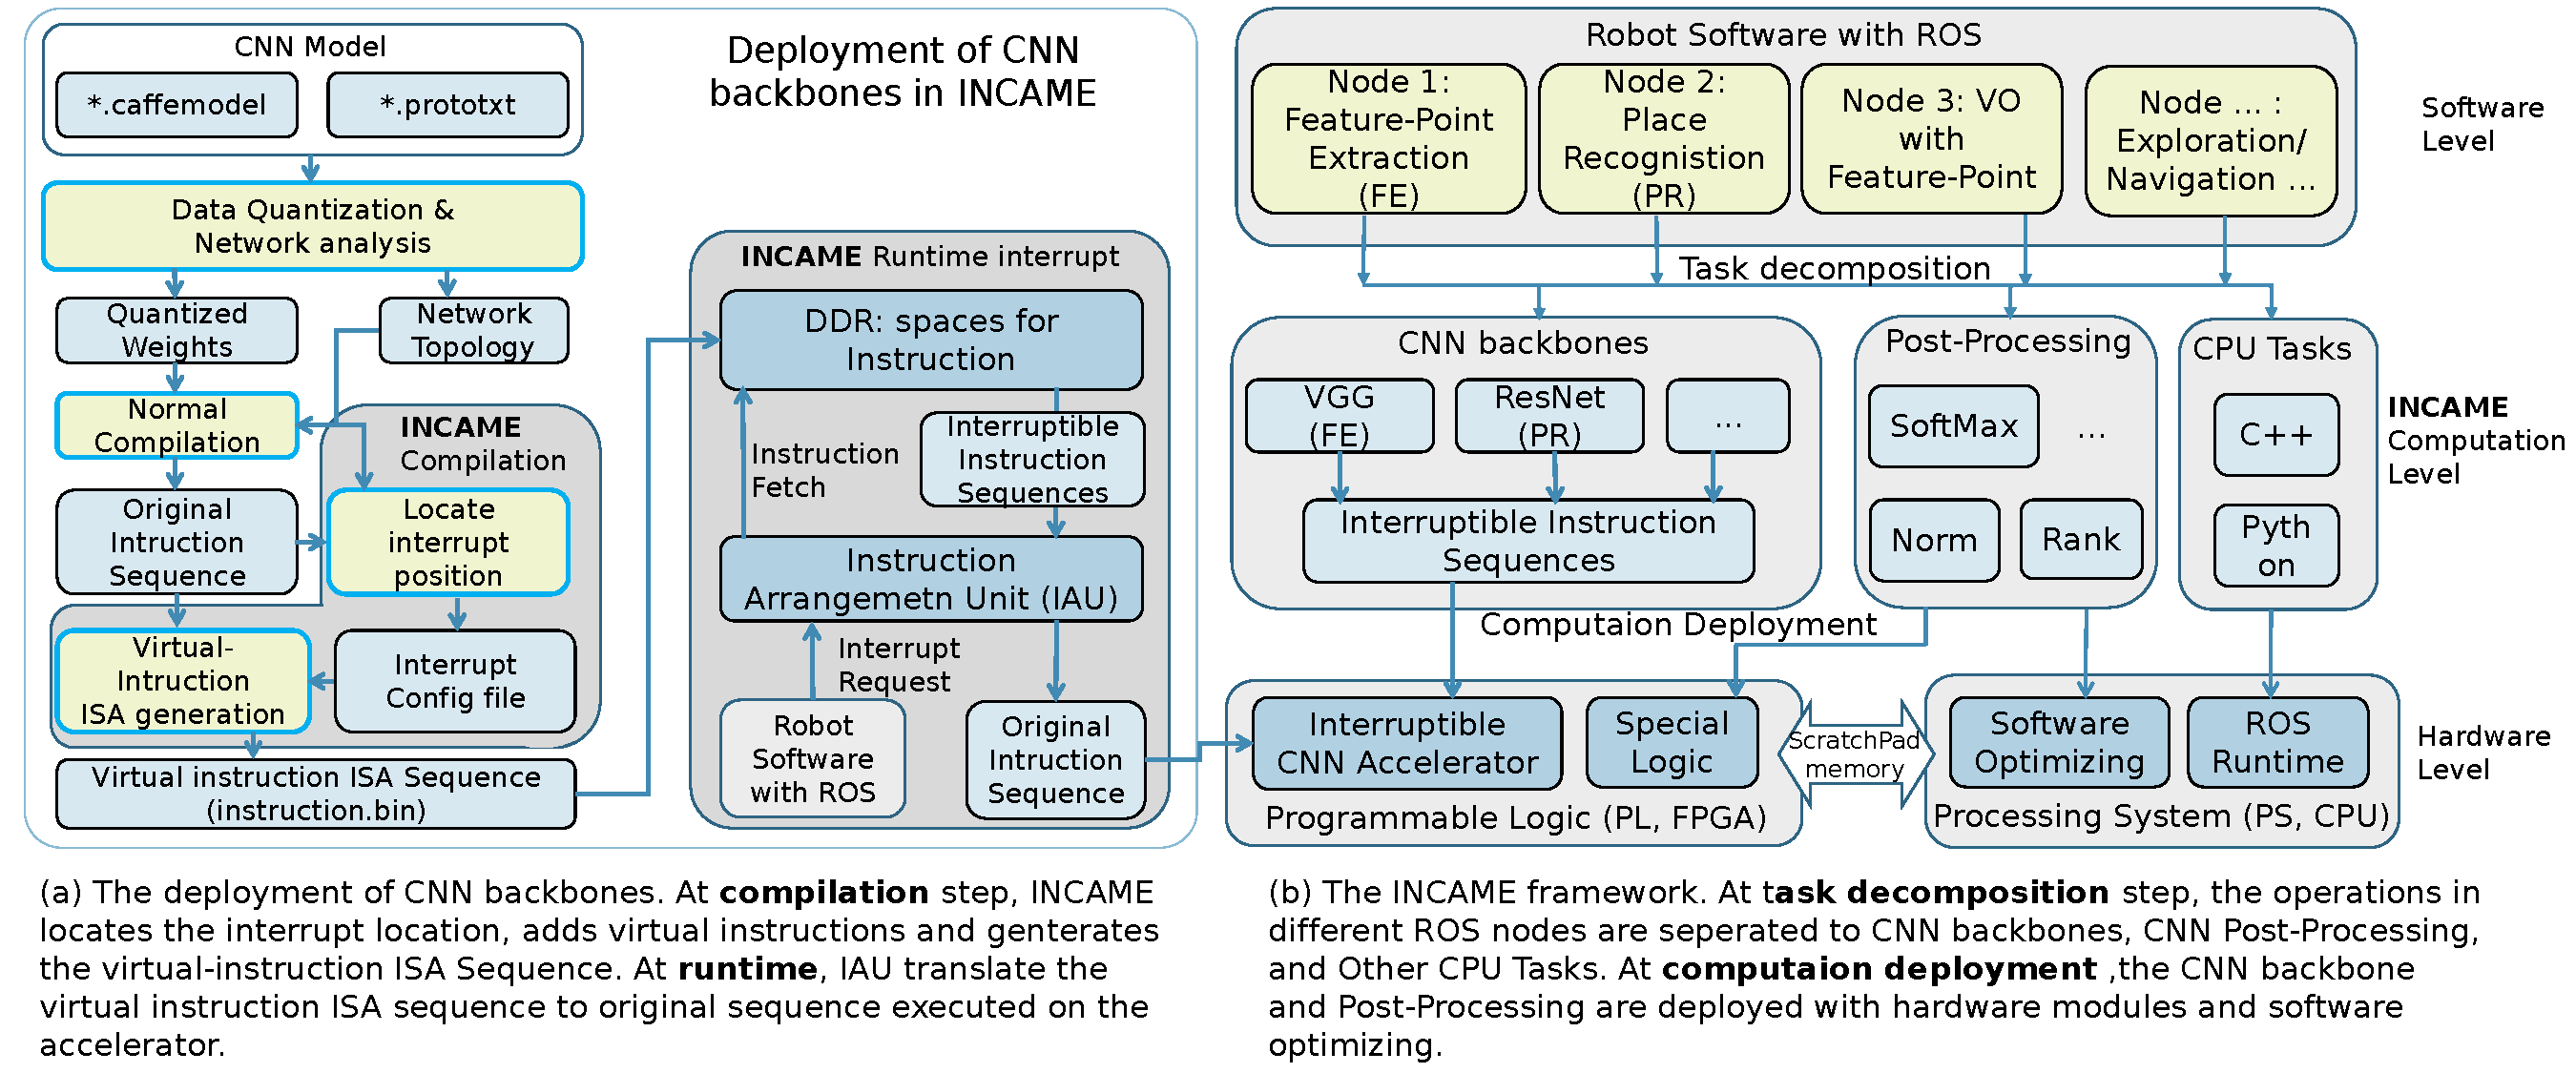
\includegraphics[width=0.99\linewidth]{fig/incame.pdf}
    \caption{ INCAME framework.}
	\label{fig:incame}
\end{figure*}


\subsection{Hardware Resources Conflicts in ROS}

Building a real robot requires many different components, including sensors, perception algorithms and control units from different developers. The Robot Operating System (ROS) \cite{quigley2009ros} is proposed to fuse the components from different researchers into a practical system. ROS is a popular framework for developing robot, which provides programming specifications and a communication interface. The modules from different developers are implemented as independent nodes in ROS. Different nodes communicate with others by topics. The publishing and subscribing nodes connect to the same topic, and neither node needs to know whether the other exists \cite{quigley2009ros}. The subscriber processes received topics through callback functions. 
Code examples of subscribing the input (key) frame topic are listed in line 17,18 in ROSExample1 and line 12,13 in ROSExample2.

Although ROS is now becoming the fundamental software platform for robotics, the independence between different ROS nodes brings \textbf{hardware resources conflicts challenge} to access the hardware accelerator. 
Because developers cannot predict the running state of the CNN accelerator when they write programs, the accelerator may be occupied by other threads when a ROS node needs to call the accelerator.
Line 13 in ROSExample1 and line 9 in ROSExample2 initialize the accelerator for each task. Line5 in ROSExample1 an d line 3 in ROSExample2 run the tasks on the same CNN accelerator respectively, which may result in hardware conflicts. 
To address this problem, the priorities of different tasks are configured at the initialization phase in INCAME.

% The run-time status of the CNN accelerator is not predictable when developers writing the program. Line 13 in ROSExample1 and line 9 in ROSExample2 initialize the DPU for each task. Line5 in ROSExample1 an d line 3 in ROSExample2 run the tasks on the same CNN accelerator, which may result in hardware conflicts. In INCAME, the priorities of different tasks are configured at initialization phase to address the hardware conflicts problem.


\begin{algorithm}[h]
    \caption{ Node for FE }
    \begin{algorithmic}[1]
        \State {\color{gray} // imagePtr, imageAddr, fmPtr, fmAddr, DPUtask, Bankendtask  is initialized by main and used in FEcallback.}
        \Function {FEcallback}{$ InputFrame $}
        \State {\color{gray} // Read and reshape the InputFrame. }
        \State {\color{blue} *imagePtr  $\gets$ *InputFrame }
        \State DPUtask.run()
        \State FEBackend.run()
        \EndFunction

        \Function {Main}{$ $}
        \State {\color{gray} // Init ScratchPad Memory. Ptr is for CPU operations, Addr is for FPGA modules.}
        \State imagePtr, imageAddr = ScratchPad(FEinputsize)
        \State fmPtr, fmAddr = ScratchPad(FEfmsize)
        \State {\color{gray}// Config task0 in IAU of the accelerator (DPU).}
        \State DPUtask = DPUinit({\color{red}  priority=0},{\color{blue} instraddr=FEinstrAddr, }
        \State \qquad \qquad \qquad \quad {\color{blue} inoffset=imageAddr,outoffset=fmAddr } ) 
        \State FEBackend = FEBackendinit({\color{blue}fmAddr, fmPtr});
        \State {\color{gray}// The node subscribes the inputframe, and use the FEcallback to process each inputframe.}
        \State Subscriber = Node.subscribe( InputFrame, FEcallback);
        \State {\color{gray}// Use spin to start the subscriber}
        \State Subscriber.spin();
        \EndFunction
    \end{algorithmic}
\end{algorithm}

\begin{algorithm}[h]
    \caption{ Node for PR }
    \begin{algorithmic}[1]
        \Function {PRcallback}{$ InputKeyFrame $}
        \State {\color{blue} *imagePtr  $\gets$ *InputKeyFrame }
        \State DPUtask.run()
        \State PRBackend.run()
        \EndFunction

        \Function {Main}{$ $}
        \State imagePtr, imageAddr = ScratchPad(PRinputsize)
        \State fmPtr, fmAddr = ScratchPad(PRfmsize)
        \State DPUtask = PR\_DPUinit( {\color{red} priority=1},{\color{blue} instraddr=PRinstrAddr}, 
        \State \qquad \qquad \qquad \quad {\color{blue} inoffset=imageAddr,outoffset=fmAddr } ) 
        \State PRBackend = PRBackendinit({\color{blue}fmAddr, fmPtr});
        \State Subscriber = Node.subscribe( InputKeyFrame, PRcallback);
        \State Subscriber.spin();
        \EndFunction
    \end{algorithmic}
\end{algorithm}



\subsection{ Interruptible Accelerator with ROS (INCAME) }

% We try to use CNN as much as possible to accomplish various tasks on the robot. Because the CNN not only has advantages over traditional algorithms in accuracy, but also has uniform and regular computing mode. Therefore, a single instruction-driven CNN accelerator can speed up different tasks. The unified accelerator can reduce the use of hardware resources and make it easier to implement the robot computing system on embedded FPGA.

\Cref{fig:incame}(b) illustrates the proposed INCAME deployment robot softwares to the embedded FPGA.
Due to advantages of CNN in image processing, more and more robot components are implemented with CNN-based method, such as feature-point extraction (FE) and place recognition (PR).
Each component is packaged as a ROS node.
The CNN backbones of ROS nodes are compiled to the  interruptible virtual instruction ISA sequences.
The task with the highest priority (FE) is not interruptible and other lower-priority tasks (PR) can be interrupted by the high-priority task. 
The post-processing of CNN-based methods, including Normalization, Rank and Softmax[??], is also accelerated in specific logic or software flow. The other tasks in C++/Python run directly on the CPU side the of embedded MPSoC\cite{MPSoC}. To eliminate the memory copy between CPU cores and CNN accelerators, we use low-latency ScratchPad memory \cite{Banakar2002Scratchpad} to directly feed the results from CNN backbones to the post-processing modules. Each shared date in ScratchPad memory is initialized with two handlers: 1) a pointer (Ptr) for the CPU thread and 2) the physical address for the hardware modules. Blue lines in  ROSExample 1,2 illustrate the usage for the ScratchPad memory.

\Cref{fig:incame}(a) shows the compilation step and run-time dynamic scheduling. Firstly, the CNN model is compiled to the normal initruction with original instruction set architecture (ISA), which is not interruptible and executed directly on the CNN accelerator.
Secondly, the compiler finds out the position to interrupt and insert the virtual buckup/recovery instructions (no virtual instructions are inserted for the highest-priority task). 
Then all the normal instructions and virtual instructions are extended to the interruptible virtual instruction ISA. At running step, an instruction arrangement unit (IAU) in hardware listens to the interrupt request from software, fetches the corresponding instructions and translates the virtual-instruction ISA to the normal ISA executed on the CNN accelerator. 
The detail of the virtual-instruction ISA and instruction arrangement unit (IAU) is introduced in \Cref{sec:cnninterrupt}.

% The design philosophy of INCAME is to use CNN as much as possible to accomplish various tasks on the robot. Because the CNN not only has advantages over traditional algorithms in accuracy, but also has uniform and regular computing mode. Therefore, a single instruction-driven CNN accelerator can speed up different tasks. The unified accelerator can reduce the use of hardware resources and make it easier to implement the robot computing system on embedded FPGA.

% The framework INCAME is proposed to make the robotics community easy to use the FPGA accelerator. As the Robot Operating System (ROS) \cite{quigley2009ros} is a popular middleware fusing different modules from different developers, INCAME is designed for the multi-thread scheduling method in ROS, as illustrated in \Cref{fig:incame}.

% In ROS, each function module is implemented as a node, and different nodes are executed in different CPU threads with asynchronous data sharing. Callback functions are used to process input data in ROS nodes. Once a ROS node subscribes to a data, and each time new data arrives, the corresponding callback function is executed.

% Each ROS node does not care about the specific execution process of the hardware accelerator (we name the accelerator DNN Processing Unit, DPU). The software only needs to configure the priority of different tasks in different nodes ( the red parameter, priority, in line 13 in ROSExample 1 and line 9 in ROSExample 2). The hardware will automatically schedule the tasks according to the priority.

% ROS is also a framework for multi-agent. Different systems with ROS can easy communicate with others.

% To eliminate the memory copy between CPU cores and CNN accelerators, we use low-latency ScratchPad memory \cite{Banakar2002Scratchpad} to directly feed the featuremaps extracted by CNN backbones to the post-processing modules. The blue lines in  ROSExample 1,2 illustrate the usage for the ScratchPad memory. Each shared date in DDR is initialized with two handlers: 1) a pointer (Ptr) for the CPU thread and 2) the physical address for the hardware modules. 
